\documentclass[12pt]{article} 

\usepackage[latin1]{inputenc}
\usepackage[spanish]{babel}
\usepackage{color}
\usepackage{multicol}
\usepackage{amsmath}
\usepackage{amssymb}
\usepackage{enumerate}
\usepackage{graphics}
\usepackage{graphicx}

\title{FLIP SORT}
\author{Sara Chica, Rodrigo Gualtero}
\date{01 de Diciembre, 2012}

\begin{document}
\maketitle
\tableofcontents

\section{Introducci�n}
Este es un problema de la UVA, identificado con el c�digo \textit{10327}, en el cual se desea saber la cantidad de pasos m�nimo para ordenar un conjunto de n�meros enteros en forma ascendente.
\\A continuaci�n se presentan 2 ejemplos de nodos:
\\
\\En el primer ejemplo se presenta un conjunto ordenado de 3 n�meros:
\begin{center}
$A=\left\{1,2,3\right\}$
\\Ejemplo 1
\end{center}
Por lo tanto no se necesitan pasos para organizarlo.
\\En el segundo ejemplo se presenta un conjunto desordenado de 3 n�meros:
\begin{center}
$B=\left\{2,3,1\right\}$
\\Ejemplo 2
\end{center}Se necesitan 2 pasos para ordenarlo.
\section{Definici�n del problema}
Este problema busca ordenar un conjunto de n�meros en forma ascendente, es decir de menor a mayor. 
\subsection{Entrada}
Entra cada uno de los casos de prueba en dos partes.
\\La primera consta de un n�mero que indica la cantidad de enteros que se deben organizar, y finalmente entran todos n�meros en el orden actual.
\subsection{Salida}
Imprime la siguiente frase: 
\begin{center}
\textsl{Minimum exchange operations : X.}
\end {center}
donde X es un entero que indica la cantidad de pasos que tuvo que hacer para organizar el vector.
\section{Modelamiento matem�tico}
Se sabe que el tren est� organizado si:
\[
Ordenado\equiv(\forall i,j | 0<i<j<100 : V_{i+1}=V_{j})
\]
Sobre este problema se podr�a extender un �rbol de posibilidades, el cual tendr�a todas las posibles permutaciones que habr�an, donde una de estas es la que satisface la condici�n de salida: Tener todos los n�meros ordenados.
\\Aplicando esto ambos ejemplos se tendr�a el siguiente �rbol de posibilidades:
\begin{center}
	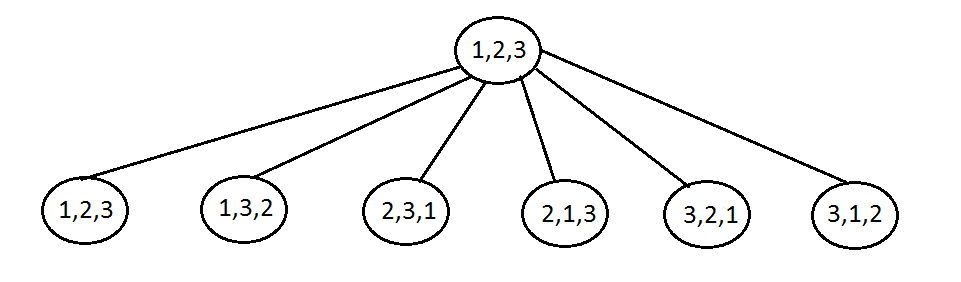
\includegraphics[width=0.50\textwidth]{Arbol.png}
	\\�rbol de posibilidades para un conjunto de 3 enteros.
\end{center}
\section{Planteamiento de la Soluci�n}
Aunque abrir un �rbol de posibilidades permite analizar mejor el problema, no es la mejor soluci�n, debido a que es poco eficiente; es por ello que existen varios algoritmos de ordenamiento, los cuales permiten organizar una lista en una secuencia dada. Para este problema se sugiere alg�n algoritmo de Intercambio, por lo cual se usar� el algoritmo burbuja.
\\Ordenamiento por Burbuja: Consiste en organizar el vector revisando cada elemento de la lista y compar�ndolo con el siguiente, de esta forma si est�n en el orden equivocado se deben intercambiar. 
\\Para el ejemplo 2 se tendr�an los siguientes pasos
\begin{center}
Origina: $A=\left\{2,3,1\right\}$
\\Paso 1: $A=\left\{2,1,3\right\}$
\\Paso 2: $A=\left\{1,2,3\right\}$
\end{center} 
\section{Conclusiones}
\begin{enumerate}
	\item Conocer los algoritmos de ordenamiento es importante para optimizar algunos otros algoritmos como los de b�squeda y fusi�n; ya que estos pueden requerir listas ordenadas para tener una ejecuci�n r�pida.
	\item El m�todo de ordenamiento burbuja es el algoritmo de ordenamiento m�s usado en los lenguajes de programaci�n, sin embargo, no es el m�s eficiente.
\end{enumerate}\end{document}